\chapter{Algorithm Development - Experimental}
\label{chapt:ALGORITHM}
\section{Premise}
The aim of the machine learning phase was to apply the Word2Vec and Doc2Vec algorithms to dataset $\Delta6$ (\S\ref{chapt:DATA_ACQUISITION}). An article was considered to be represented by a document consisting of its title and abstract. The aim was to represent these documents as vectors in semantic space, so that advanced computational analyses and statistical methods could be performed. This section constitutes an experimental section.
\section{Data Sanitisation} 
The documents (titles and abstracts) in $\Delta6$ required preprocessing before they could be effectively used in training. The training process requires inputs to be as clean as possible in order to get good results (encapsulated by the well-known computer science idiom `Garbage in, Garbage out'). 

The first step was to cast all words to lower case, so that the algorithm did not produce different vectors for e.g.  `Molecule' and `molecule'.

The raw documents also frequently contained artefacts from the source webpages (unwanted whitspace, vestigial HTML tags, `newline' characters and carriage returns). The algorithm training word vectors for these symbols is clearly undesired behaviour, so these were removed and whitespace normalised.

It was also observed that, as unicode text scraped from a wide variety of sources, there was varied and redundant punctuation. Punctuation would be treated as separate words by the algorithm, so had to be carefully removed. Unicode has very wide variety of different punctuations. For example, unicode encodes 24 different types of hyphen. Table \ref{fig:punct} shows the punctuation that was filtered out of the documents. Large sections of unicode script (sections of non-western languages) was also removed as the algorithm works best on a smaller vocabulary.

\begin{figure}[H]
    \centering
    \textbf{Filtered Punctuation }\par\medskip
    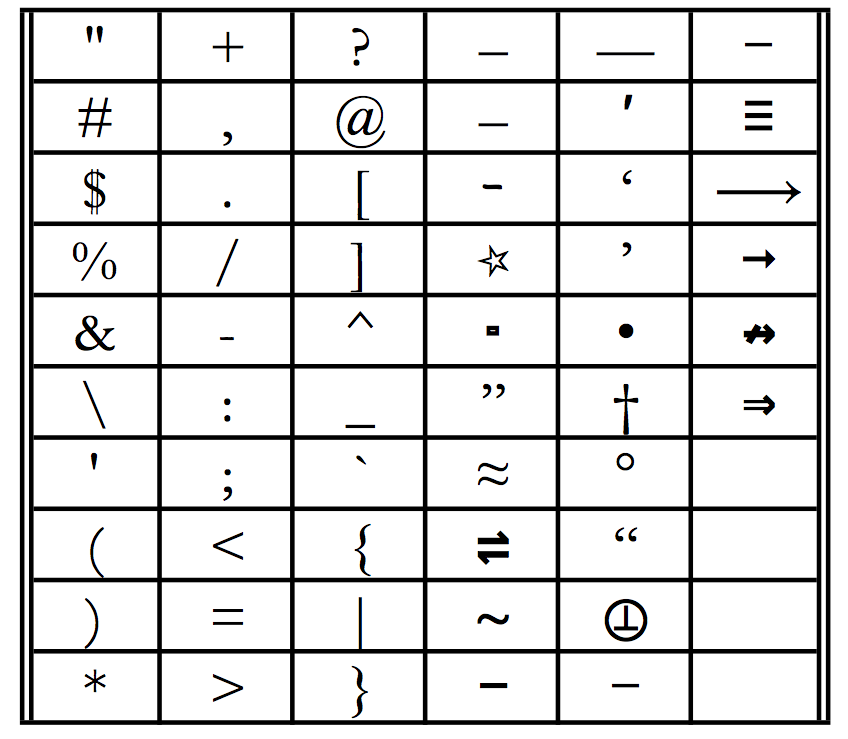
\includegraphics[scale=0.2]{Algorithm/punct_table.png}
    \caption[Punctuation removed in sanitation processing]{All the punctuation removed in sanitation. Only these were found in appreciable quantities in the $\Delta6$. }
     \label{fig:punct}
\end{figure}
Removing hyphens and primes also meant chemical names were fragmented. This was considered acceptable as the fragment words had greater freedom than specific (possibly singleton) fully-formed names, e.g. \texttt{5-methyl-1-heptanol} is split to \texttt{5 methyl 1 heptanol}, this allows the \texttt{heptanol} fragment to be associated with other mentions of heptanol in the training set, rather than only associate with mentions of the much less frequent 5-methyl-1-heptanol. 

Next, English stopwords were removed\footnote{Stopwords are commonly occurring words in a corpus that hold little information, e.g. (`the', `a', `and'...), see glossary} \footnote{stopwords were taken from the Porter stopwords corpus\cite{nltk},\cite{porter}}. From inspection of the zipfian frequency table, (\S \ref{sec:CORPUSOBSERVATIONS}), it was apparent that chemistry literature also has stopwords. Table \ref{tab:CHEMSTOP} details `Chemistry' stopwords that were identified and removed\footnote{The chemistry stopwords were chosen from high on the rank frequency table (they appeared extremely commonly) and because they were considered to encode little information; for instance, the digits appeared so frequently and in such an wide set of contexts, no meaningful vector would be trained. The word structure appeared so frequently, so as to encode very little actual information.}. 
\begin{table}[H]
\begin{center}
\caption{Chemistry stopwords}
\label{tab:CHEMSTOP}
\begin{tabular}{||c|c|c|c|c||}
\hline
chemistry & containing & 7 & six & water\\
structure & novel & 8 & seven & also\\
structural & study & 9 & eight & method\\
study & studies & 0 & nine & molecular\\
new & 1 & zero & ten & studied\\
using & 2 & one & phase& \\
based & 3 & two & based& \\
reaction & 4 & three & compounds & \\
reactions & 5 & four & high & \\
chemical & 6 & five & results & \\
\hline

\end{tabular}
\end{center}
\end{table}

Finally, the processed words were sent through a `stemming algorithm'\footnote{A stemming algorithm seeks to map derived words onto the same root, such as polymer and polymers, but some also attempt more complex cases such as morphologic and morphology}. Several stemming algorithms were assessed (Porter\cite{porter}, Snowball\cite{snowball}\cite{nltk}, Lancaster \cite{lancaster} and the Wordnet Lemmatizer \cite{wordnet1}\cite{wordnet2}\cite{wordnet3}). The Snowball\footnote{Also known as Porter2.} stemmer was found to strike a good balance between making an appreciable number of contractions (superior to Wordnet) whilst minimising conflations and over-contraction (superior to Lancaster and Porter). See Table \ref{tab:stems}
\begin{table}[H]
\begin{center}
\caption{Stemming Comparisons}
\label{tab:stems}
\begin{tabular}{||c|c|c|p{5cm}||}
\hline
Word & Porter Stemmed & Snowball Stemmed & Comment\\
\hline     
phyllenthus & phyllenthu & phyllenthus & Overagressive stemming by Porter\\
\hline
angularly & angularli & angular & Adverbs map to root better\\
\hline
infinitly & infinitli & infinit & \multirow{2}{5cm}{Snowball maps these to correct root}\\
\cline{1-3}
infinite & infinit & infinit&\\
\hline
\hline
Word & Lancaster Stemmed & Snowball Stemmed & Comment\\
\hline
pigment & pig & pigment & Lancaster collapses too far\\
\hline
conductive & conduc & conduct & \multirow{2}{5cm}{Lancaster conflates these different words}\\
\cline{1-3}
conducive & conduc & conduct & \\
\hline
scripting & scripting & script & Lancaster doesn't consider present participles\\
\hline
aroma & arom & arom & \multirow{2}{5cm}{Preferable not to map aroma and aromatic to same root}\\
\cline{1-3}
aromatic & arom & aromat & \\
\hline
\end{tabular}
\end{center}
\end{table}

The document preprocessing pipeline is shown diagrammatically in figure \ref{fig:SANPIPE}:

\begin{figure}[H]
    \centering
    \textbf{Preprocessing pipeline}\par\medskip
  \makebox[\textwidth][c]{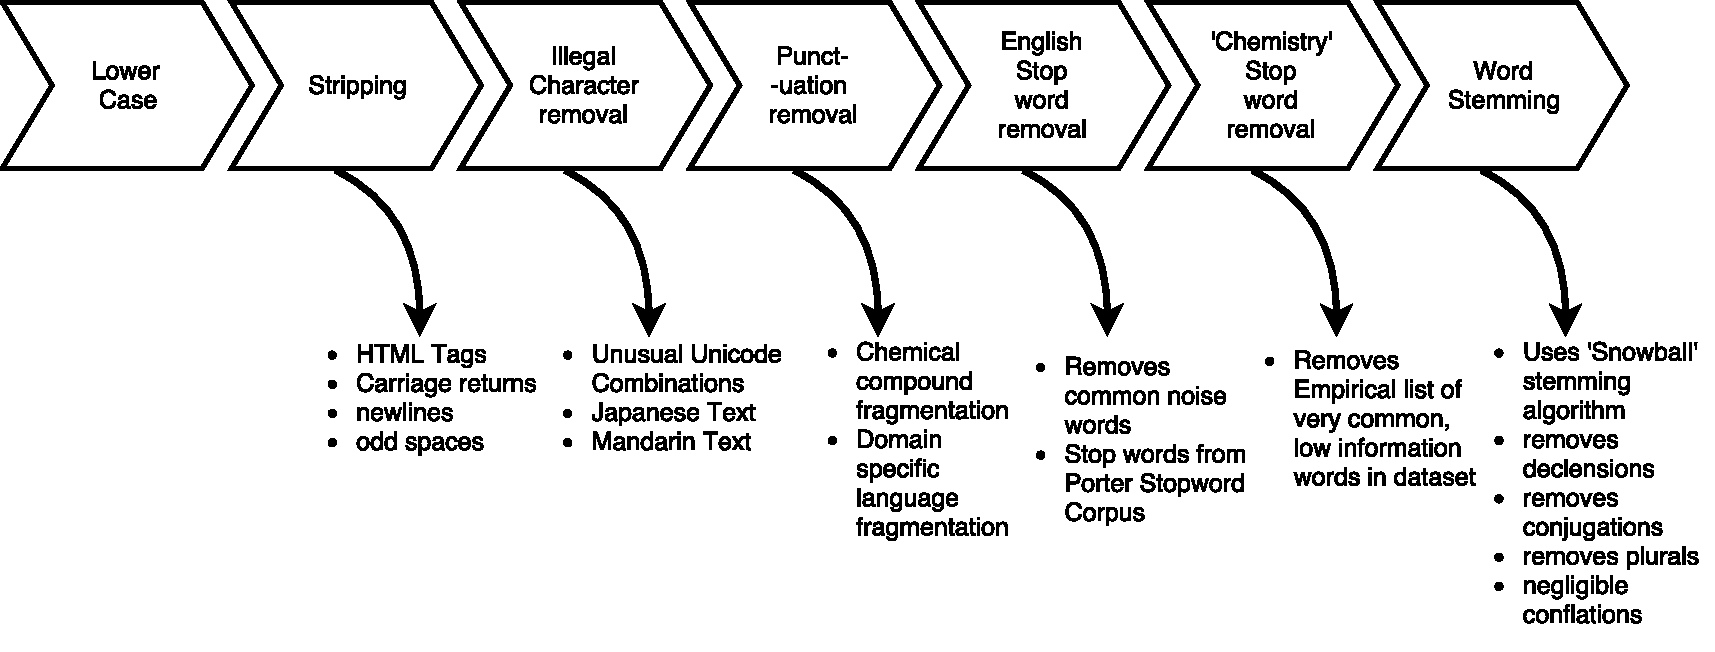
\includegraphics[width=1.15\textwidth]{Algorithm/Data_Sanitation-2.pdf}}%
    \caption[Preprocessing Pipeline]{All documents in $\Delta6$ were preprocessed with this pipeline schema before being used in training models}
     \label{fig:SANPIPE}
\end{figure}
The process is best illustrated by real example from $\Delta6$:

$<$ p $>$
\texttt{ n A 9-silafluorene-containing biphenolic monomer,\\ 9,9-bis(4-hydroxyphenyl)-9-silafluorene,\\ was prepared from 9,9-dichloro-9-silafluorene and employed for the \\synthesis of polyesters using a fluorene-based homoditopic acid chloride.} $< \setminus$ p $>$.
\cite{sanex} 

processed into:

\texttt{silafluoren biphenol monom bis hydroxyphenyl silafluoren prepar dichloro\\ silafluoren employ synthesi polyest fluoren homoditop acid chlorid}

Whilst challenging to read, word order is preserved and low information words (or words with complex, diverse meanings such as numbers) have been removed to give good-quality input data. Note how chemical names have been fragmented so that multiple chemical vectors can be learned, rather than the fewer complex vectors (\texttt{\\9,9-dichloro-9-silafluorene} vs \texttt{dichloro} and \texttt{silafluoren}).

\section{Word2Vec Models}
The processed data was used to train two Word2Vec models (one CBOW, one skipgram) using the gensim implementation\cite{gensim}. The hyperparameters used for training were consistent for the two models.
Training was carried out on all documents in $\Delta6$. The model was trained with sentences formed by simple splitting of documents using full stops\footnote{Whilst not perfect, this method was a fair compromise for partitioning on actual sentences and false partitioning.}. After examination of different hyperparameters, the models were run using hyperparameters representing good balance of specificity, speed and generality. The hyperparameters used are detailed in table \ref{tab:hyperparams}.
\begin{table}[H]
\begin{center}
\caption{Word2vec Parameters}
\label{tab:hyperparams}

\begin{tabular}{||c|c||}
\hline
Model Parameter &CBOW and skipgram\\
\hline
Vector Dimensionality & 100\\
Minimum word frequency & 1 (all words)\\
Initial learning rate $\alpha$ & 0.025 \\
Minimum learning rate $\alpha_{min}$&0.0001\\
Epochs of training & 24\\
Sliding word window size & 5\\
Negative sampling & Yes \\
Downsampling parameter & 0.001\\
Hierarchical Softmax & No\\
CBOW Mean & Yes (Not applicable for Skipgram) \\
\hline
\end{tabular}
\end{center}
\end{table}
In order to represent documents as vectors using these models, the component word vectors had to be aggregated into a single vector. There were several possible aggregation techniques, described below.
\subsection{TF-IDF}
TF-IDF\footnote{Term - frequency Inverse - Document - Frequency} is an empirical metric for weighting the importance of words in a sentence. If averaging word vectors, it is intuitive that equal weighting should not be given to information heavy and trivial words. The TF-IDF weight, defined as term frequency: $TF \left( w , d \right) = f_{ w \in d }$ where $f\left( w \right)$ is the raw frequency of a term $w$ in a document d,
multiplied by inverse document frequency $IDF(w) = log_{2} \left( \frac{|D|}{\sum_d df_{w \in d})} \right)$ where $|D|$ is the number of documents in the corpus, $df$ is 1 if word $w$ is in document $d$, otherwise 0\cite{gensim}.
TF-IDF assigns small weights to words that are common across the corpus. It assigns high weights to words that appear often in a document but rarely in the corpus.
\subsection{Aggregations}
Document vectors could be created by averaging word vectors into sentence vectors, followed by averaging sentence vectors into document vectors, or by simpy averaging word vectors directly into documents. 8 models for document vectors composed of Word2Vec models were constructed, detailed in table \ref{tab:aggmods}
\begin{table}[h!]
\begin{center}
\caption{Word2vec Document Vector Models}
\label{tab:aggmods}
\begin{tabular}{||L|p{3.8cm}|N|p{3.8cm}||}
\hline
Model Name & Description & Model Name & Description\\
\hline
CBOW-W & Simple average of CBOW word vectors & SG-W & Simple average of skipgram word vectors\\
\hline
CBOW-S & CBOW word vectors averaged to sentence vectors, then sentence vectors averaged & SG-S & SG word vectors averaged to sentence vectors, then sentence vectors averaged\\
\hline
CBOW-TFIDF-W & CBOW-W with TFIDF weighting on word vectors & SG-TFIDF-W & SG-W with TF-IDF weighting on word vectors. \\
\hline
CBOW-TFIDF-S & CBOW-S with TFIDF weighting on word vectors & SG-TFIDF-S & SG-S with TF-IDF weighting on word vectors\\
\hline
\end{tabular}
\end{center}
\end{table}

\section{Doc2Vec Models}
A Doc2Vec model was trained with a \emph{distributed memory} architecture\footnote{Distributed memory is the Paragraph Vector algorithm equivalent of CBOW, the performance of this architecture is optimal\cite{doc2vec}} using the gensim framework in Python \cite{gensim} using $\Delta6$ with the same sanitation pipeline as for the Word2Vec models. The training sentences were labelled with the document (journal article DOI) they came from. 100 dimensional vectors were chosen as a compromise of training speed and specificity\footnote{as well as for computational considerations of analytical techniques, see \S\ref{chapt:VALIDATION},\S\ref{chapt:ANALYSIS}}, and also so that dimensions were consistent across all models. The Doc2Vec model was trained for 24 epochs, with hyperparameters detailed in table \ref{tab:doc2vechyperparams}
\begin{table}[H]
\begin{center}
\caption{Word2vec Parameters}
\label{tab:doc2vechyperparams}
\begin{tabular}{||c|c||}
\hline
Model Parameter & value\\
\hline
Vector Dimensionality & 100\\
Minimum word frequency & 1 (all words)\\
Initial learning rate $\alpha$ & 0.025 \\
Minimum learning rate $\alpha_{min}$&0.0001\\
Epochs of training & 24\\
Sliding word window size & 8\\
Negative sampling & No \\
Hierarchical Softmax & Yes\\
CBOW Mean & Yes (Not applicable for Skipgram) \\
\hline
\end{tabular}
\end{center}
\end{table}

The model took considerably longer to train than Word2Vec, as there were appreciably more work required per  document. Negative sampling was disabled as per recommendations in the literature\cite{gensim} \cite{doc2vec}.
The Doc2Vec and Word2Vec models are assessed in \S\ref{chapt:VALIDATION}.
